% !TeX spellcheck = en_US

% some nice styling for code listings
\definecolor{mygreen}{rgb}{0,0.6,0}
\definecolor{mygray}{rgb}{0.5,0.5,0.5}
\definecolor{mymauve}{rgb}{0.58,0,0.82}

\lstset{ %
	backgroundcolor=\color{white},   % choose the background color; you must add \usepackage{color} or \usepackage{xcolor}
	basicstyle=\footnotesize,        % the size of the fonts that are used for the code
	breakatwhitespace=false,         % sets if automatic breaks should only happen at whitespace
	breaklines=true,                 % sets automatic line breaking
	captionpos=b,                    % sets the caption-position to bottom
	commentstyle=\color{mygreen},    % comment style
	deletekeywords={...},            % if you want to delete keywords from the given language
	escapeinside={\%*}{*)},          % if you want to add LaTeX within your code
	extendedchars=true,              % lets you use non-ASCII characters; for 8-bits encodings only, does not work with UTF-8
	frame=no,	                   % adds a frame around the code
	keepspaces=true,                 % keeps spaces in text, useful for keeping indentation of code (possibly needs columns=flexible)
	keywordstyle=\color{blue},       % keyword style
	language=Octave,                 % the language of the code
	otherkeywords={*,...},           % if you want to add more keywords to the set
	numbers=left,                    % where to put the line-numbers; possible values are (none, left, right)
	numbersep=5pt,                   % how far the line-numbers are from the code
	numberstyle=\tiny\color{mygray}, % the style that is used for the line-numbers
	rulecolor=\color{black},         % if not set, the frame-color may be changed on line-breaks within not-black text (e.g. comments (green here))
	showspaces=false,                % show spaces everywhere adding particular underscores; it overrides 'showstringspaces'
	showstringspaces=false,          % underline spaces within strings only
	showtabs=false,                  % show tabs within strings adding particular underscores
	stepnumber=2,                    % the step between two line-numbers. If it's 1, each line will be numbered
	stringstyle=\color{mymauve},     % string literal style
	tabsize=2,	                   % sets default tabsize to 2 spaces
	title=\lstname                   % show the filename of files included with \lstinputlisting; also try caption instead of title
}

% helper for importing csv files with underscores
\DeclareUrlCommand\UScore{\urlstyle{rm}}
\newcommand{\expUScore}{%
	\expandafter\expandafter\expandafter
	\UScore
	\expandafter\expandafter\expandafter
}

\chapter{Simple demo \sbml models}
\section{Simple demo SBML version1}
\label{sec:appendix:simple-demo:v1}
\lstinputlisting[language=XML]{../supplementary/demo-sbml-simple/version1.xml}

\section{Simple demo SBML version2}
\label{sec:appendix:simple-demo:v2}
\lstinputlisting[language=XML]{../supplementary/demo-sbml-simple/version2.xml}

\chapter{Render of Delta between a more advanced demo model}
\begin{figure}[h]
	\centering
	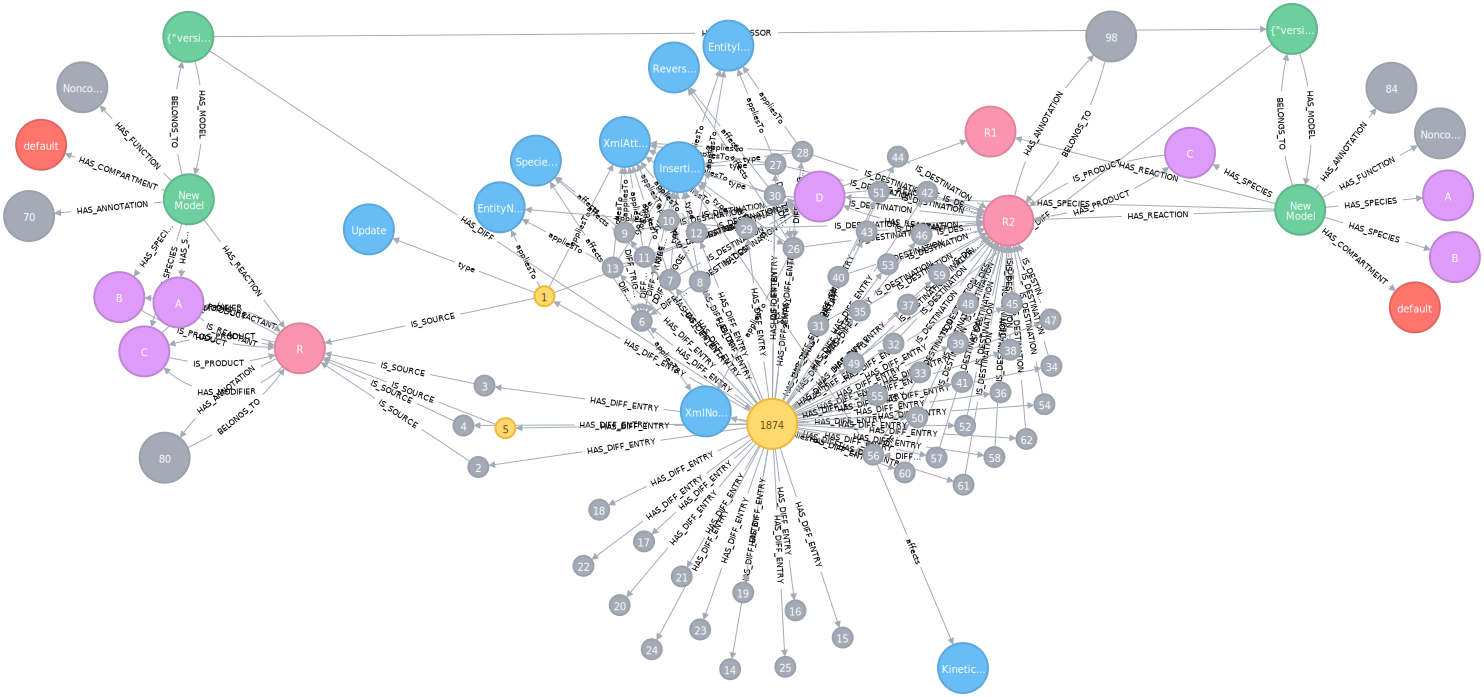
\includegraphics[width=\textwidth]{resources/neo4j-renders/demo-sbml-diff.pdf}
	\caption{\neoj graph representation of a delta between two demo models}
	\label{fig:appendix:demo-sbml-diff}
\end{figure}

\chapter{Representation of \comodi in \masymos}
\begin{figure}[h]
	\centering
	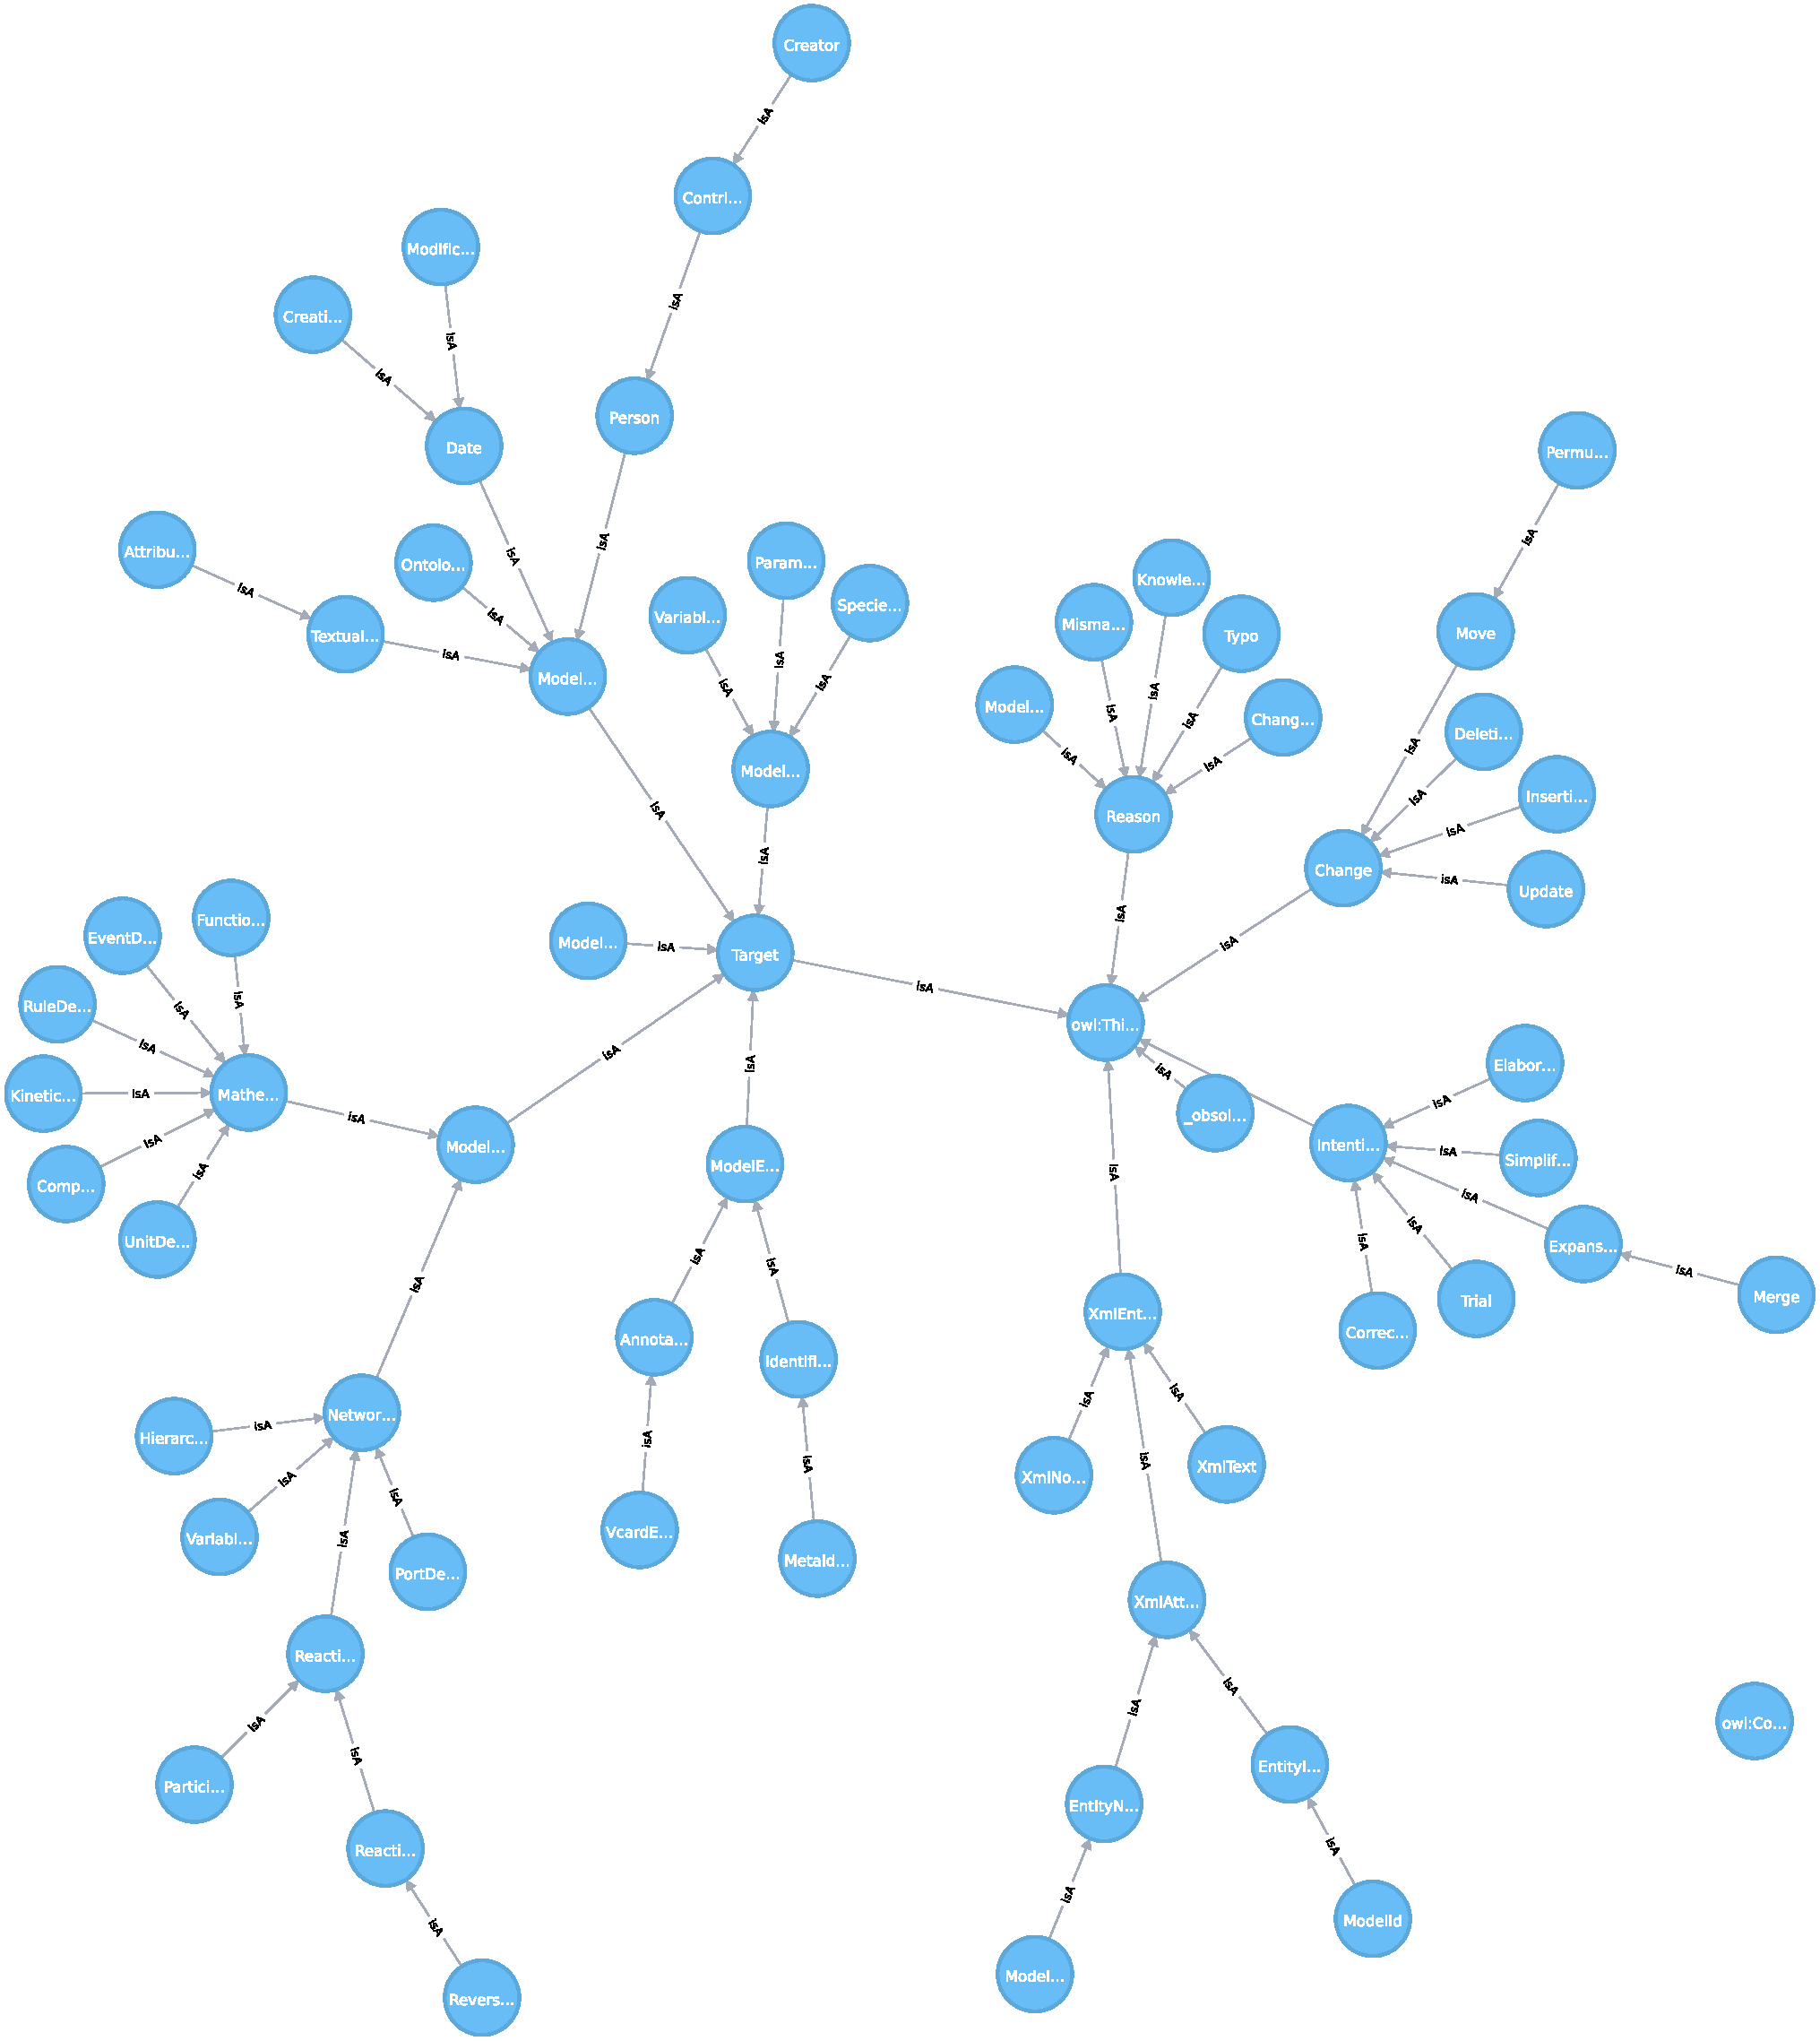
\includegraphics[width=\textwidth,height=0.5\textheight,keepaspectratio]{resources/neo4j-renders/comodi.pdf}
	\caption{Representation of \comodi in \masymos/\neoj}
	\label{fig:appendix:neo4j-comodi}
\end{figure}

\chapter{Overview of Node- and Relationship types}
\todo{tables are ugly as hell...}
\todo{write introduction thingy, where these numbers are coming from}

\section{Graphical Overview}
\begin{figure}[H]
	\centering
	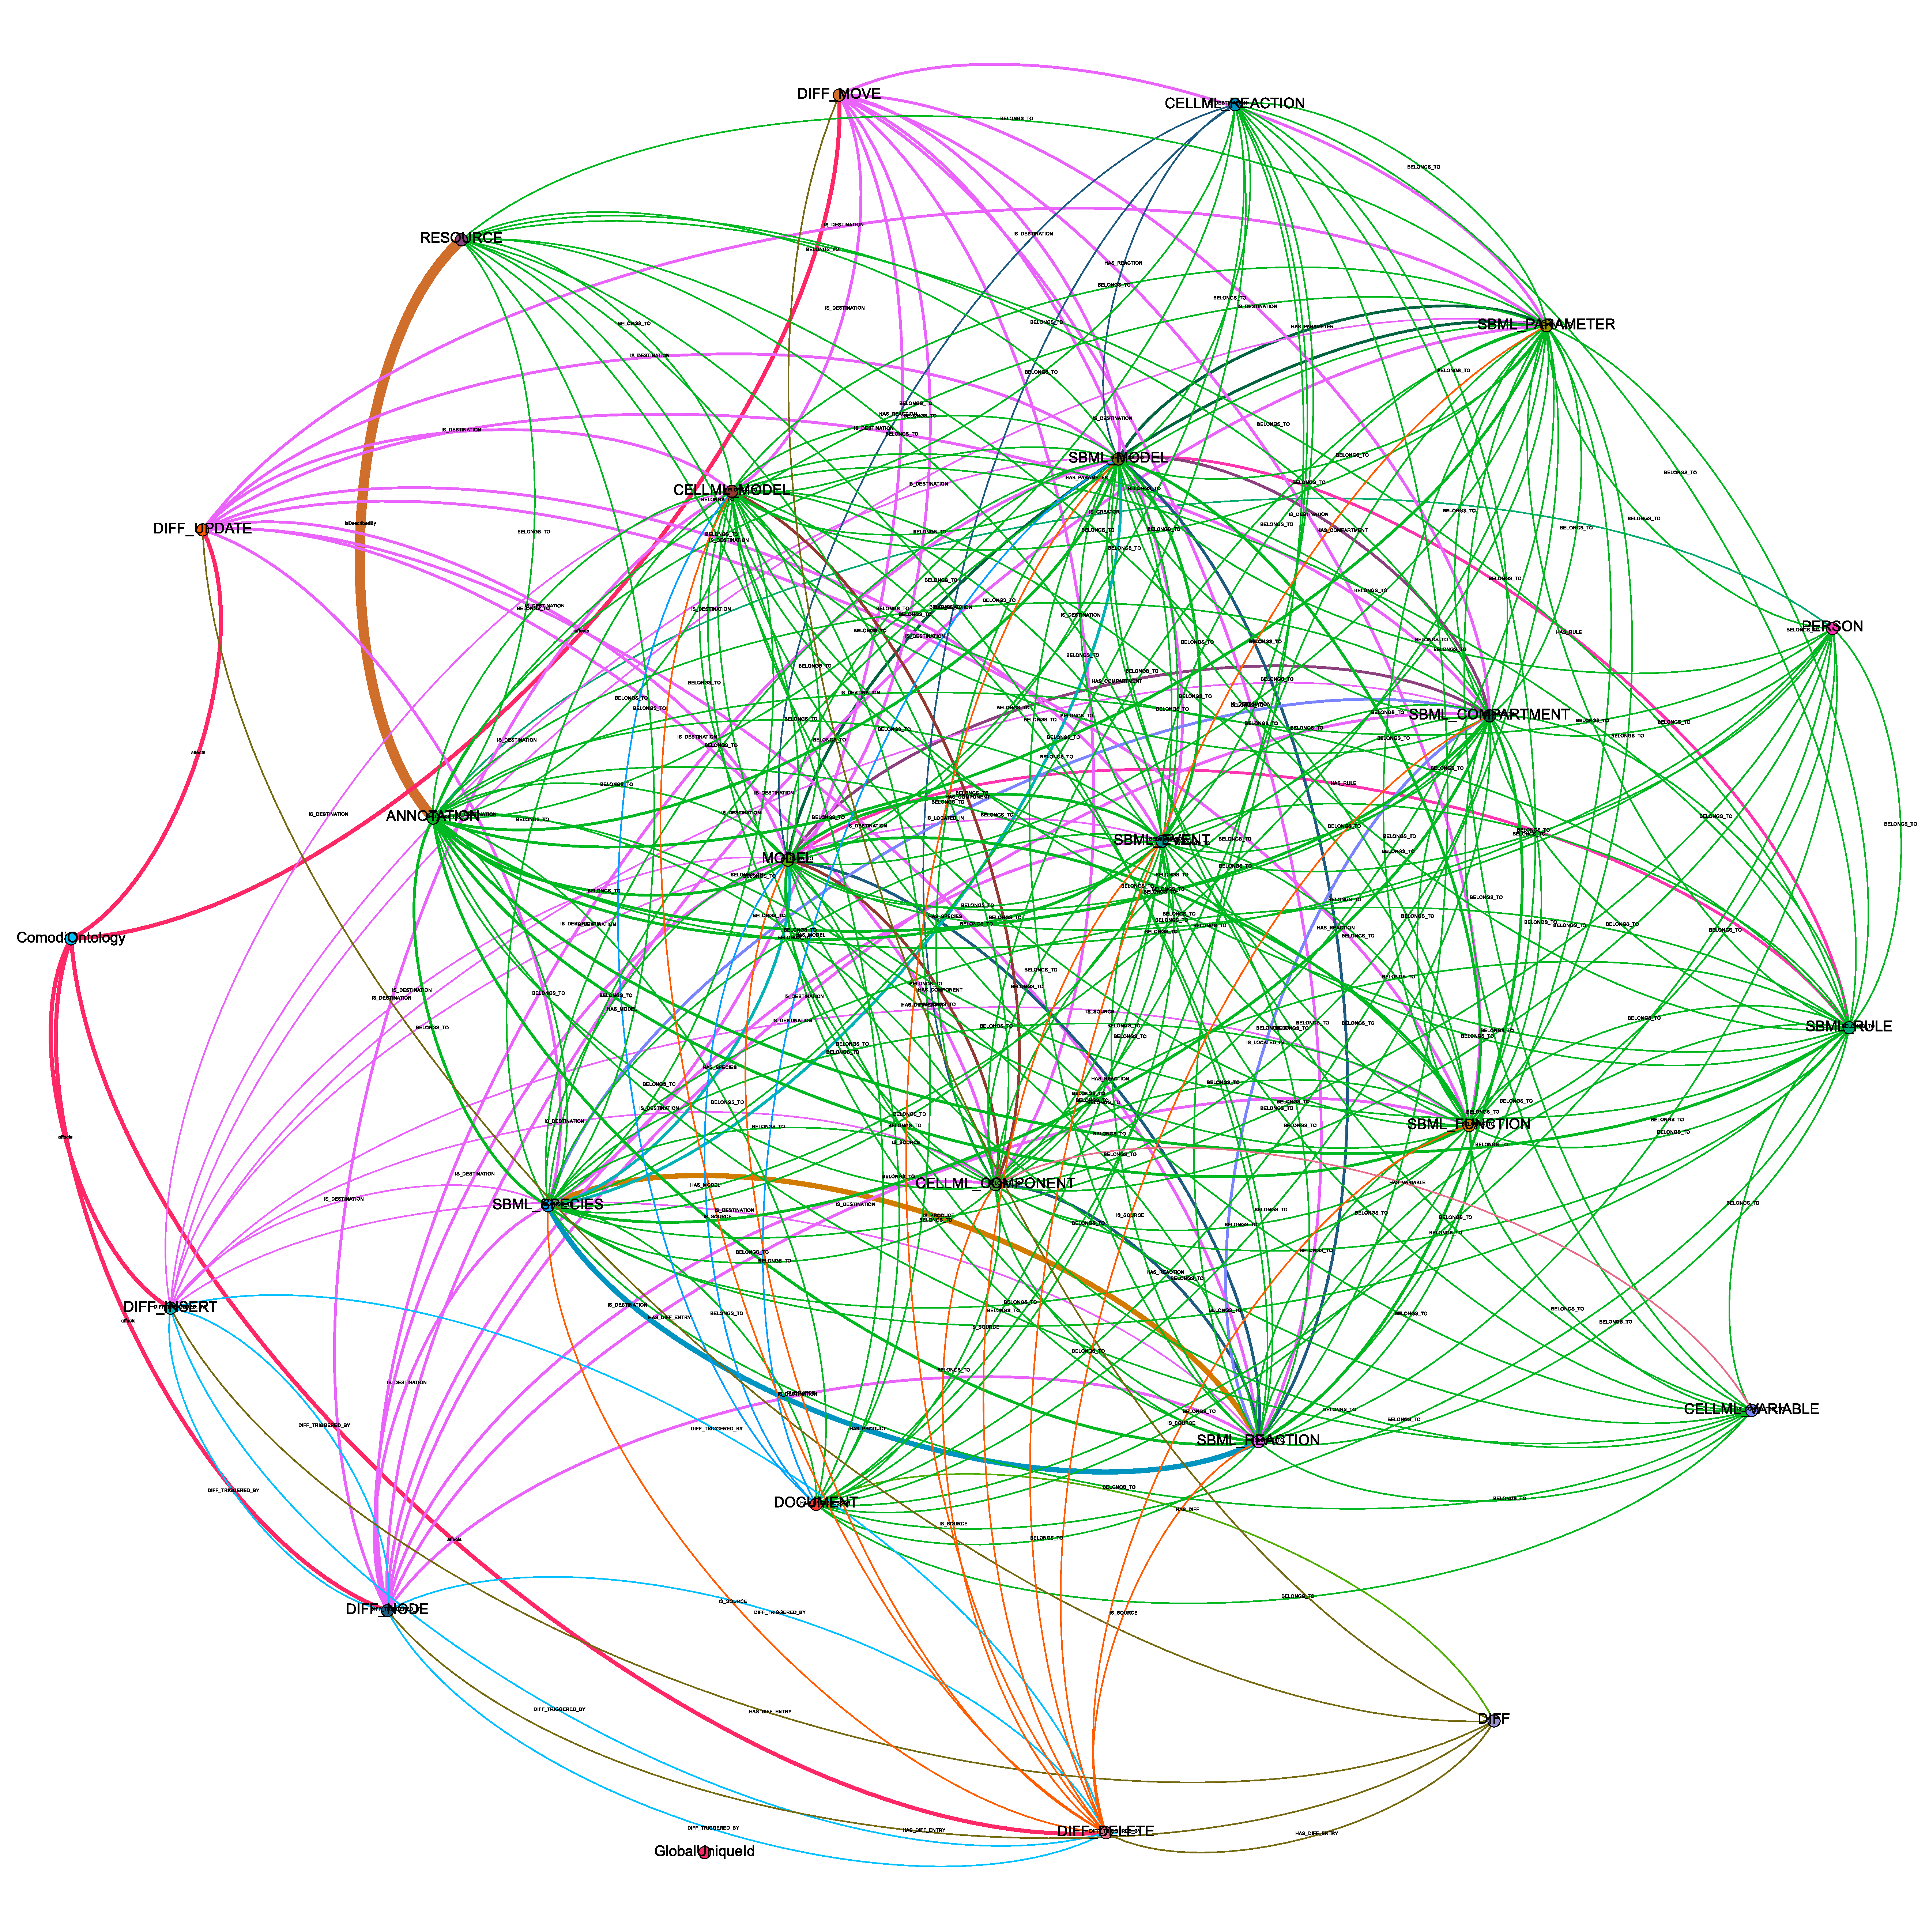
\includegraphics[width=\textwidth,height=0.5\textheight,keepaspectratio]{resources/neo4j-renders/large-test-meta-graph.pdf}
	\caption{Overview of all used node types and relations between them}
	\label{fig:appendix:meta-graph}
\end{figure}

\section{List of all used Node types}
\begin{longtable}{ l r }
	\hline \bfseries Node Label & \bfseries No. of occurrence \\\hline \endhead
	\csvreader[head to column names]{resources/neo4j-renders/large-test-meta-graph-nodes.csv}{} %
	{\expUScore{\label} & \count \\} %
	%\hline
\end{longtable}

\section{List of all used Relationship types}
\begin{longtable}{ l c r r }
	\hline \bfseries Source Node Label & \bfseries Relationship Type & \bfseries Destination Node Label \\\hline \endhead %
	\csvreader[]{resources/neo4j-renders/large-test-meta-graph-edges-expanded.csv}{Source=\sourceNode,Target=\targetNode,label=\relLabel,count=\count} %
	{\expUScore{\sourceNode} & \expUScore{\relLabel} & \expUScore{\targetNode}\\} %
	%\hline
\end{longtable}
